\chapter{\REVIEW{License Plate Recognition}}
\label{chap:license-plate-recognition}

License plate detection is an task in computer vision that involves identifying and localizing license plates within images or videos. 
This task has numerous practical applications, such as automated toll collection, parking management, and law enforcement. 
To perform license plate detection, various AI models have been developed that use computer vision techniques. 
In this research, we will compare four such models and recommend the most suitable one based on their performance, accuracy, suitability, and load. 
These models have been selected based on a review of the article \cite{lic:license-plate}.

\section{Image processing}

    \subsection{Edge detection for license plate recognition}

    Edge detection is a fundamental technique in computer vision used to extract edges from an image. 
    In license plate recognition, edge detection can be used to extract the boundaries of the license plate, which can then be used for further processing such as character segmentation and recognition.

    There are several edge detection algorithms that can be used for license plate recognition, such as Sobel, Canny, and Roberts. 
    However, Canny edge detection is the most commonly used algorithm due to its superior performance in detecting edges with low noise sensitivity and high accuracy.
    \cite{egde:edge-dection}

    \textbf{Canny edge detection works using the following steps:}

        \begin{enumerate}

        \item \textbf{Gaussian smoothing}

        The first step is to apply Gaussian smoothing to the image to reduce noise and obtain a smoother image. 
        This is done by convolving the image with a Gaussian filter kernel.

        \item \textbf{Gradient calculation}

        The second step is to calculate the gradient of the smoothed image using a derivative operator such as Sobel or Roberts. 
        The gradient represents the rate of change of intensity in the image and can be used to detect edges.

        \item \textbf{Non-maximum suppression}

        The third step is to apply non-maximum suppression to the gradient image to thin out the edges and obtain a one-pixel-wide edge map. 
        This is done by selecting the local maximum in the direction perpendicular to the edge and setting all other pixels to zero.

        \item \textbf{Double thresholding}

        The fourth step is to apply double thresholding to the edge map to classify each edge pixel as either strong or weak. 
        This is done by comparing each pixel intensity with two thresholds: a high threshold and a low threshold. 
        Pixels with intensity above the high threshold are classified as strong edges, pixels with intensity below the low threshold are classified as non-edges, and pixels with intensity between the two thresholds are classified as weak edges.

        \item \textbf{Edge tracking by hysteresis}

        The fifth and final step is to perform edge tracking by hysteresis to link weak edges into strong edges. 
        This is done by starting at a strong edge pixel and following the adjacent weak edge pixels until no more weak edges are found. 
        This process is repeated for all strong edge pixels until all edges are connected.

        \end{enumerate}

\section{Machine learning}

    \subsection{Haar-cascade}
    Haar-cascade is a object detection algorithm that was developed by Viola and Jones in 2001. 
    The algorithm is based on the Haar wavelet technique, which is a mathematical concept used to detect image features. 
    The Haar-cascade algorithm is widely used for face detection, but it can also be used for other object detection tasks.
    \cite{hrcs:haar-cascades}

        \textbf{The Haar-cascade algorithm works uses the following steps:}
        \begin{enumerate}
            
            \item \textbf{Haar Feature Selection}
        
            The first step in the Haar-cascade algorithm is to select a set of features that are used to detect the object. 
            Haar features are rectangular features that are used to represent the object. In figure \ref{fig:haar_features_example} is a example of how the haar features look. 
            The algorithm selects the best set of features that can distinguish between the object and the background.

            \begin{linfigure}{fig:haar_features_example}{Example of the haar features}
                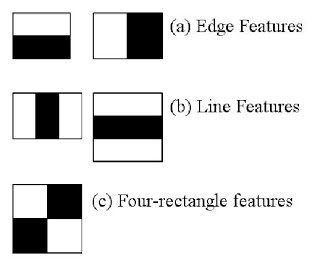
\includegraphics[width=0.5\textwidth]{haar_features_example}
            \end{linfigure}
                
            \item \textbf{Integral Image}
        
            The second step is to calculate the integral image of the input image. The integral image is a matrix of the same size as the input image, where each element represents the sum of all the pixels above and to the left of it. 
            The integral image is used to speed up the calculation of the Haar features. 
            The value of a pixel at location $(x,y)$ in the integral image can be defined as the cumulative sum of all the pixels in the rectangular region defined by the upper-left corner at $(0,0)$ and the lower-right corner at $(x,y)$:
            
            I(x,y)=∑i=0x∑j=0yP(i,j)
            I(x,y)=i=0∑x​j=0∑y​P(i,j)
            
            where $P(i,j)$ is the value of the pixel at location $(i,j)$. This cumulative sum includes the value of the pixel at $(x,y)$ itself, as well as all the pixels to its left and above it.
            In figure \ref{fig:integral_image_example}, there is example of how a integral image will look like.

            \begin{linfigure}{fig:integral_image_example}{Example of how intergral images works}
                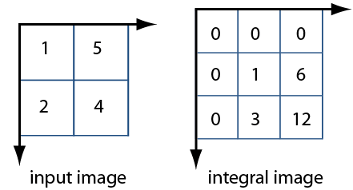
\includegraphics[width=0.5\textwidth]{integral_image_example}
            \end{linfigure}
            
            \item \textbf{Adaboost Training}
        
            The third step is to train an Adaboost classifier using the selected Haar features. 
            Adaboost is a machine learning algorithm that combines weak classifiers to create a strong classifier. 
            The Haar features are used as weak classifiers, and the Adaboost algorithm trains the classifier to minimize the false positives and false negatives.
        
            \item \textbf{Cascade Classifie}
        
            The fourth step is to create a cascade classifier using the trained Adaboost classifier. 
            The cascade classifier consists of multiple stages, where each stage contains a set of classifiers. 
            The output of each stage is a binary decision that determines whether the object is present or not. 
            The cascade classifier is used to reduce the number of false positives by quickly rejecting the input that is not likely to contain the object.

        \end{enumerate}

    \subsection{HOG + Linear SVM}
    The Histogram of Oriented Gradients (HOG) is a feature extraction technique used for object detection in computer vision. 
    HOG computes the distribution of edge orientations in an image and is an effective feature descriptor for object detection.

    Linear Support Vector Machines (SVMs) are a type of supervised learning algorithm that can classify input data into one of two categories based on a set of features. 
    SVMs are often used in combination with HOG features for object detection.
    \cite{hgms:hog-multiscale}

        \textbf{The HOG + Linear SVM algorithm works uses the following steps:}
        \begin{enumerate}

            \item \textbf{Image Preprocessing}
        
            The first step in the HOG + Linear SVM algorithm is to preprocess the image by resizing it to a fixed size, converting it to grayscale, and performing contrast normalization. 
            These steps help to reduce the variations in lighting and color in the image, making it easier to detect objects.
            
            \item \textbf{Compute HOG features}
        
            The next step is to compute the HOG features for the image. 
            HOG features are computed by dividing the image into small cells, computing the gradient orientation for each pixel in the cell, and then creating a histogram of gradient orientations for each cell. 
            The histogram values are then normalized and concastenated to form a feature vector.

            \item \textbf{Training the Linear SVM}
        
            After computing the HOG features for the training images, the next step is to train a Linear SVM using these features. 
            The Linear SVM learns a decision boundary that separates the positive (object) examples from the negative (non-object) examples.
        
            The training process involves minimizing the classification error subject to a regularization parameter that controls the trade-off between maximizing the margin and minimizing the classification error.
        
            \item \textbf{Sliding Window Detection}
        
            Once the Linear SVM is trained, the next step is to use it for object detection in test images. 
            The HOG feature extraction process is applied to a sliding window of the test image at multiple scales and positions.
        
            At each window position, the HOG features are computed, and the Linear SVM is used to classify the window as either containing an object or not. 
            If the window is classified as containing an object, it is considered a detection.

            \item \textbf{Non-Maximum Suppression}
        
            Finally, the algorithm performs Non-Maximum Suppression (NMS) to remove duplicate detections and retain only the most confident detections. 
            NMS involves selecting the detection with the highest confidence score and removing all other detections that overlap with it by more than a certain threshold.

        \end{enumerate}

    \subsection{YOLO}
    YOLO is an acronym for 'You Only Look Once'. It is an algorithm that can detect and recognize various objects. 
    YOLO performs object detection as a regression problem and provides the class probabilities of the detected images.

    The YOLO algorithm employs convolutional neural networks (CNN) to detect objects in real-time. 
    As the name suggests, the algorithm requires only a single forward propagation through a neural network to detect objects.

    This means that prediction for the entire image is done in a single algorithm run. 
    The CNN is used to predict various class probabilities and bounding boxes simultaneously.
    \cite{ylalgo:yolo-algorithm}

        \textbf{The YOLO algorithm works uses the following steps:}
        \begin{enumerate}

            \item \textbf{Residual blocks}
        
            The first step is to divide the original image (A) into equal-shaped grid cells of size NxN, where N=4 in this case (as shown in figure \ref{fig:yolo_grid_example} bellow). 
            Each cell in the grid is responsible for localizing and predicting the class of the object that it covers, along with a probability/confidence value.

            \begin{linfigure}{fig:yolo_grid_example}{Example of how to image is split up in grids}
                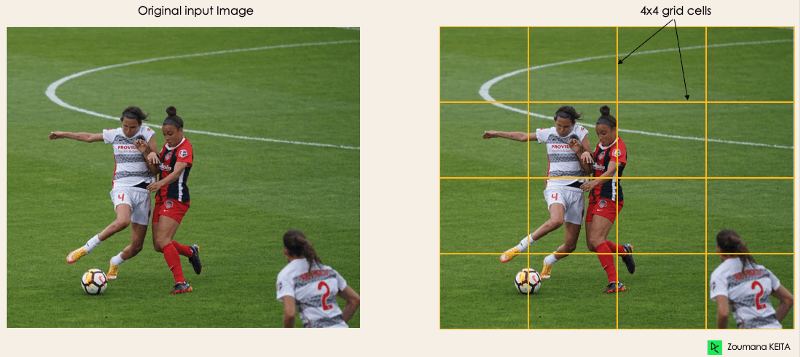
\includegraphics[width=0.5\textwidth]{yolo_grid_example}
            \end{linfigure}
            
            \item \textbf{Bounding box regression}
        
            The next step is to detect the objects in an image and determine the bounding boxes that correspond to each object. 
            YOLO uses a single regression module to determine the attributes of each bounding box in the following format, where \(Y\) represents the final vector representation for each bounding box: \(Y = [pc, bx, by, bh, bw, c1, c2]\)
        
            The values in the \(Y\) vector are crucial during the training phase of the YOLO model.

            \begin{itemize}
            \item The \(pc\) value represents the probability score of the grid cell containing an object. For example, in an image with several objects, all the grid cells containing an object will have a probability score higher than zero, while the grid cells without an object will have a probability score of zero.
            \item The \(bx\) and \(by\) values represent the x and y coordinates of the center of the bounding box with respect to the enveloping grid cell.
            \item The \(bh\) and \(bw\) values represent the height and width of the bounding box with respect to the enveloping grid cell.
            \item The \(c1\) and \(c2\) values correspond to the different classes of objects to be detected. In the example of a soccer game, c1 might represent the class "player," and c2 might represent the class "ball." YOLO can detect as many classes as required for a given use case.
            \end{itemize}

            \item \textbf{Intersection Over Unions or IOU}
        
            When detecting an object in an image using YOLO, multiple grid boxes can overlap with the object, even though not all of them are relevant. 
            The IOU (Intersection over Union) metric is used to filter out irrelevant grid boxes and retain only those that are relevant.
        
            First, the user defines an IOU selection threshold, such as 0.5. 
            YOLO then calculates the IOU for each grid cell by dividing the area of intersection by the area of union between the grid cell and the object.
            
            Finally, YOLO disregards any grid cells with an IOU value less than or equal to the threshold and only considers those with an IOU value greater than the threshold.
        
            \item \textbf{Non-Max Supression or NMS}
        
            Setting an IOU threshold alone may not always be sufficient when detecting objects in an image using YOLO, as an object can have multiple bounding boxes with an IOU value beyond the threshold. 
            Keeping all of these boxes can result in noise and reduce the accuracy of the detection.
        
            To address this issue, YOLO employs Non-Maximum Suppression (NMS), which selects only the bounding box with the highest probability score of detection for each object. 
            This approach ensures that only the most likely bounding box is retained for each object, while discarding the others with lower probability scores.

        \end{enumerate}

    \subsection{SSD (Single Shot MultiBox Detector)}
    SSD is a real-time object detection algorithm that can detect multiple objects in an image using a single pass through a deep neural network. 

    The SSD algorithm uses a pre-trained convolutional neural network to predict bounding boxes and class probabilities for the objects present in an image. 
    It does this by dividing the input image into a grid of fixed-size cells, and then predicting the class probabilities and bounding box offsets for each cell.
    \cite{ssdalgo:SSD-algorithm}

        \textbf{The SSD algorithm works uses the following steps:}
        \begin{enumerate}

            \item \textbf{Feature extraction}
        
            The first step in the SSD algorithm is to extract features from the input image using a pre-trained convolutional neural network (CNN). 
            The CNN takes in the input image and produces a feature map, which is a 3D tensor of shape \((H, W, C)\), where H and W are the height and width of the feature map, and C is the number of channels.
            
            \item \textbf{Multiscale feature maps}
        
            SSD uses multiple feature maps of different resolutions to detect objects of different sizes. 
            This is achieved by adding additional convolutional layers to the base CNN and creating feature maps of different resolutions. 
            The SSD algorithm then applies a set of convolutional filters to each feature map to predict bounding boxes and class probabilities for each cell.

            \item \textbf{Anchor boxes} 
        
            To handle objects of different aspect ratios and sizes, the SSD algorithm uses anchor boxes. 
            Anchor boxes are predefined bounding boxes of different aspect ratios and sizes that are used as a reference during object detection. 
            For each cell in the feature map, the SSD algorithm predicts offsets for the anchor boxes, which are used to calculate the final bounding box coordinates.
        
            \item \textbf{Non-Maximum Suppression or NMS} 
        
            The final step in the SSD algorithm is non-maximum suppression (NMS), which eliminates duplicate detections and selects the most accurate bounding boxes for each object. 
            NMS works by selecting the bounding box with the highest class probability and eliminating any other bounding boxes that have a high overlap (measured using IOU) with the selected box.

        \end{enumerate}